\documentclass[DIV=11, a4paper, parskip=true]{scrartcl}
\RequirePackage{listings}
\RequirePackage{graphicx}
\RequirePackage[british]{babel}
\RequirePackage{float}
\RequirePackage{booktabs}
\RequirePackage{longtable}
\RequirePackage{color}

% Default fixed font does not support bold face
\DeclareFixedFont{\ttb}{T1}{txtt}{bx}{n}{10} % for bold
\DeclareFixedFont{\ttm}{T1}{txtt}{m}{n}{10}  % for normal

% Custom colors
\definecolor{deepblue}{rgb}{0,0,0.5}
\definecolor{deepred}{rgb}{0.6,0,0}
\definecolor{deepgreen}{rgb}{0,0.5,0}

% Python style for highlighting
\lstset{
language=Python,
basicstyle=\ttm,
otherkeywords={self},             % Add keywords here
keywordstyle=\ttb\color{deepblue},
emph={MyClass,__init__},          % Custom highlighting
emphstyle=\ttb\color{deepgreen},    % Custom highlighting style
stringstyle=\color{deepred},
showstringspaces=false,           % 
breaklines=true,
prebreak=\raisebox{0ex}[0ex][0ex]{\ensuremath{\hookleftarrow}}
}

\author{Grzegorz Lippe\\
{\small \texttt{grzegorz@posteo.de}}}
\title{Explore Weather Trends}
\subtitle{Udacity Data Analyst Project}
\date{30\textsuperscript{th} of March 2020}
\begin{document}
\maketitle

\begin{abstract}
This document is a analysis of local and global temperature data and comparison of
the temperature trends of Munich to overall global temperature trends.

It gives a visualization and a written up description of the similarities and differences
between global temperature trends and Munich.
\end{abstract}

\tableofcontents

\pagebreak
\section{Extracting the Data}
The data was extracted and exported to CSV from the Udacity projects website. The SQL queries
used where:

\lstset{language=SQL, basicstyle=\ttm, numbers=left}
\begin{lstlisting}[caption=SQL queries]
select * from global_data;
select year, avg_temp from city_data where city='Munich';
\end{lstlisting}

The first statement in line 1 selects all data in \texttt{global\_data}, which after inspection
showed to be two columns, one a year and the other one the global average temperature in
$^\circ$C. So the first dataset is complete.

The second statement selects the year and corresponding average temperature for the city of
Munich from the table \texttt{city\_data} which is the closest big city to my home.

Munich was chosen after inspection of the table \texttt{city\_list}, which showed that 3
German cities are included in the city data. A second inspection of city data showed, that
there are additional columns present, namely: country and city. These were not selected in
the SQL Query in line 2, since this information is not needed for the upcoming analysis.

Both queries where executed and saved as \texttt{global\_data.csv} and
\texttt{munich\_data.csv}.

\pagebreak
\section{Manipulating the Data}

Since I'm familiar with Python and Pandas I chose these tools to manipulate the data.
The following listing shows the method I used to import \texttt{global\_data.csv}

\begin{lstlisting}[language=Python, caption=Import the data from \texttt{global\_data}]
global_data = pd.read_csv('global_data.csv',
    names=['Year', 'Yearly Global Average Temperature'],
    index_col='Year',
    header=0)

for window in [5, 10, 20]:
    global_data['%d years global moving average temperature' % (window)] =\
        global_data['Yearly Global Average Temperature'].rolling(window=window).mean()

_, ax = plt.subplots(figsize=(14, 8))
global_data.plot(ax=ax, title='Global (moving) average Temperatures')
plt.ylabel('Average Temperature [C]')
plt.grid(True)
plt.savefig('./global_average_temperatures.png')
\end{lstlisting}

In the first four lines the csv data is imported and cast into a Pandas DataFrame. I chose to
use the year as an index for the DataFrame. This is beneficial, because the index is used for
the abscissa values within the DataFrame plot method.

In the lines 6 to 8 a for loop is used to add columns with [5, 10, 20] years of moving average.
The moving average is calculated by a combination of the DataFrame Methods \texttt{rolling()}
and the numpy method \texttt{mean()}.

In the last lines 10ff a figure is created, which shows the contents of the DataFrame. These
are the global average temperature and the three moving averages within the time span. It is
from the 1750s up until 2015.

The resulting plot is shown in Figure~\ref{global_averages}.

\begin{figure}[H]
    \centering
    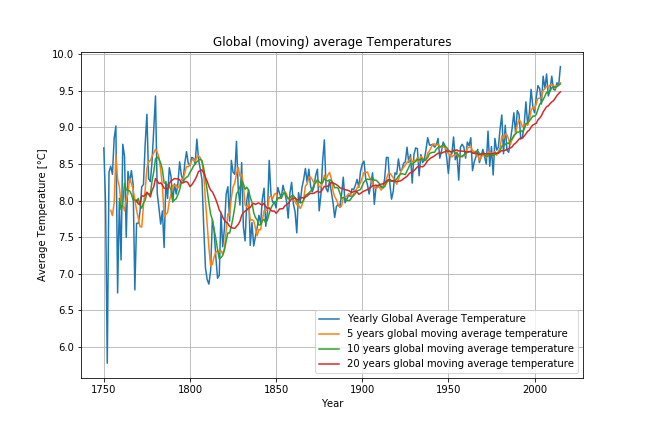
\includegraphics[width=0.7\columnwidth]{global_average_temperatures.png}
    \caption{Earth's average temperatures}
    \label{global_averages}
\end{figure}

It can be seen, that the 5 years moving average isn't very smooth, yet the 20 years moving
average is so smooth, that it misses the cold period in the 1820's quite a bit. So therefore a
10 years moving average is chosen.

The same methodology is used for the Munich's data and yields the following
Figure~\ref{munich_averages}.

\begin{figure}[H]
    \centering
    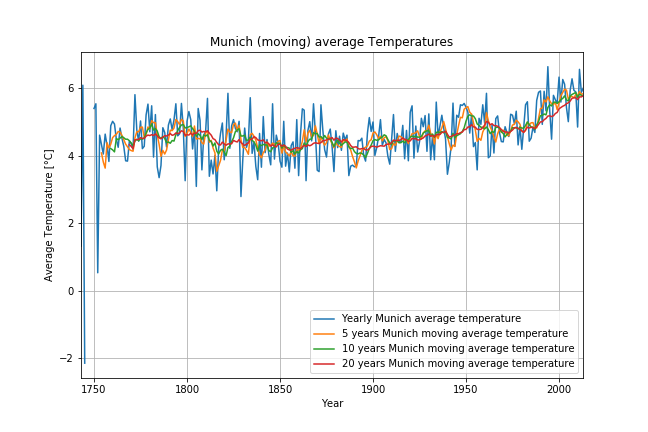
\includegraphics[width=0.7\textwidth]{munich_average_temperatures.png}
    \caption{Munich's average temperatures}
    \label{munich_averages}
\end{figure}

From this plot it is already clear, that the temperature data of munich seems to be more
steady.

\pagebreak
\section{Create Clear Data Visualization}

Goal of this work is to make observations about the similarities and differences between the
world averages and Munich's averages, as well as overall trends. Therefore two additional
figures are introduced, to compare the world and Munich's data.

Figure \ref{comparison} shows the global and Munich's 10 years moving average temperature
combined in one plot. The dates range from the late 1750s to 2015. The temperatures range from
roundabout $4^\circ$C to $9.5^\circ$C.

\begin{figure}[H]
    \centering
    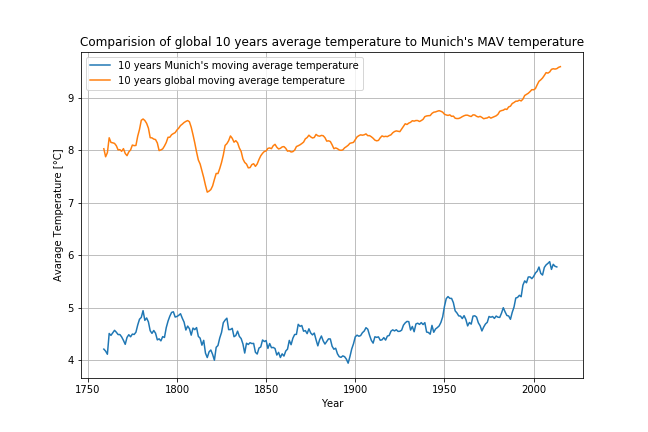
\includegraphics[width=0.9\textwidth]{comparison_average_temperatures.png}
    \caption{Absolute average temperature comparison}
    \label{comparison}
\end{figure}

From Figure~\ref{comparison} it is difficult to see similarities because the global temperature
is roundabout two times higher thant the moving average temperature of Munich.

Therefore in Figure~\ref{rel_comparison} the values where normalized. Both moving average
datasets start at 1759, so the value of that year was taken to divide both temperatures series
by it and thereby setting these years values to 100\%.

\begin{figure}[H]
    \centering
    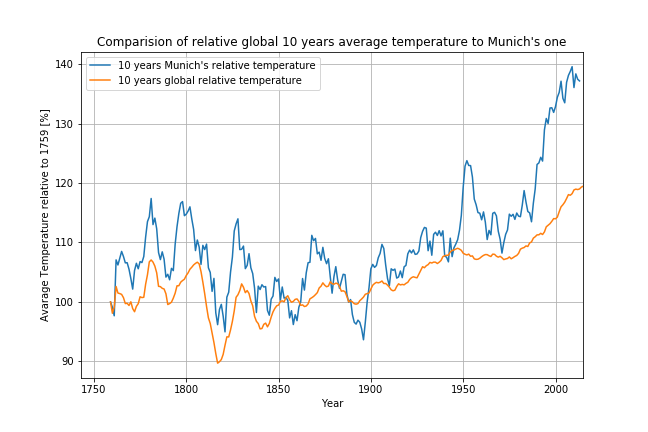
\includegraphics[width=0.9\textwidth]{rel_comparison_average_temperatures.png}
    \caption{Relative average temperature comparison}
    \label{rel_comparison}
\end{figure}

\section{Interpret Weather Trends}

This section provides (at least four) observations, which I provide, drawn from my own
visualizations.

\begin{itemize}
\item Figure \ref{global_averages} show that the global year averages where fluctuating around
$8^\circ$C up until the 1920s.
\item Figure \ref{global_averages}, or Figure \ref{comparison} also show, that the global
yearly average temperature increased by roundabout 1.5$^\circ$C in the last 100 years.
\item There seems to have been a pause in the global temperature increase from the 1950s until
the 1970s.
\item The comparison Figure~\ref{comparison} show that the global average temperature is
roundabout double of Munich's temperatures.
\item The overall spikes and valleys in both data sets matches.
\item Figure~\ref{rel_comparison} shows that the global temperature is roughly 20\% higher than
1759 and the Munich temperature is roughly 35\% higher than in 1759.
\item A detailed inspection of the data showed extreme low temperatures in the years of 1743,
1745 and 1752, where the average temperature in Munich was $1.32^\circ$C, $-2.15^\circ$C and $0.53^\circ$C, see
annex Table~\ref{csv_data}. These could be due to the measurement equipment in the
18\textsuperscript{th} century, but the global data of also shows a spike at 1752 of $5.78^\circ$C.
\end{itemize}

\begin{longtable}{lrr}
\caption{Raw CSV data, joined} \\
\label{csv_data} \\
\toprule
{} &  Munich &  Global \\
Year &         &         \\
\midrule
\endhead
1743 &    1.32 &     NaN \\
1744 &    6.09 &     NaN \\
1745 &   -2.15 &     NaN \\
1746 &     NaN &     NaN \\
1747 &     NaN &     NaN \\
1748 &     NaN &     NaN \\
1749 &     NaN &     NaN \\
1750 &    5.40 &    8.72 \\
1751 &    5.54 &    7.98 \\
1752 &    0.53 &    5.78 \\
1753 &    4.61 &    8.39 \\
1754 &    4.33 &    8.47 \\
1755 &    4.05 &    8.36 \\
1756 &    4.64 &    8.85 \\
1757 &    4.30 &    9.02 \\
1758 &    3.83 &    6.74 \\
1759 &    4.89 &    7.99 \\
1760 &    5.02 &    7.19 \\
1761 &    4.94 &    8.77 \\
1762 &    4.49 &    8.61 \\
1763 &    4.25 &    7.50 \\
1764 &    4.82 &    8.40 \\
1765 &    4.52 &    8.25 \\
1766 &    4.28 &    8.41 \\
1767 &    3.85 &    8.22 \\
1768 &    3.84 &    6.78 \\
1769 &    4.43 &    7.69 \\
1770 &    4.36 &    7.69 \\
1771 &    4.19 &    7.85 \\
1772 &    5.81 &    8.19 \\
1773 &    4.76 &    8.22 \\
1774 &    4.43 &    8.77 \\
1775 &    5.03 &    9.18 \\
1776 &    4.21 &    8.30 \\
1777 &    4.28 &    8.26 \\
1778 &    5.21 &    8.54 \\
1779 &    5.53 &    8.98 \\
1780 &    4.71 &    9.43 \\
1781 &    5.48 &    8.10 \\
1782 &    3.96 &    7.90 \\
1783 &    5.22 &    7.68 \\
1784 &    3.67 &    7.86 \\
1785 &    3.35 &    7.36 \\
1786 &    3.71 &    8.26 \\
1787 &    4.83 &    8.03 \\
1788 &    4.69 &    8.45 \\
1789 &    4.26 &    8.33 \\
1790 &    4.91 &    7.98 \\
1791 &    5.09 &    8.23 \\
1792 &    4.77 &    8.09 \\
1793 &    5.06 &    8.23 \\
1794 &    5.54 &    8.53 \\
1795 &    4.59 &    8.35 \\
1796 &    4.65 &    8.27 \\
1797 &    5.55 &    8.51 \\
1798 &    4.81 &    8.67 \\
1799 &    3.26 &    8.51 \\
1800 &    5.02 &    8.48 \\
1801 &    5.31 &    8.59 \\
1802 &    5.07 &    8.58 \\
1803 &    4.20 &    8.50 \\
1804 &    4.80 &    8.84 \\
1805 &    3.09 &    8.56 \\
1806 &    5.40 &    8.43 \\
1807 &    5.05 &    8.28 \\
1808 &    3.58 &    7.63 \\
1809 &    4.61 &    7.08 \\
1810 &    4.72 &    6.92 \\
1811 &    5.70 &    6.86 \\
1812 &    3.39 &    7.05 \\
1813 &    3.87 &    7.74 \\
1814 &    3.46 &    7.59 \\
1815 &    4.01 &    7.24 \\
1816 &    2.96 &    6.94 \\
1817 &    4.21 &    6.98 \\
1818 &    4.66 &    7.83 \\
1819 &    4.97 &    7.37 \\
1820 &    3.88 &    7.62 \\
1821 &    4.59 &    8.09 \\
1822 &    5.85 &    8.19 \\
1823 &    4.22 &    7.72 \\
1824 &    4.89 &    8.55 \\
1825 &    5.07 &    8.39 \\
1826 &    4.81 &    8.36 \\
1827 &    4.71 &    8.81 \\
1828 &    5.02 &    8.17 \\
1829 &    2.79 &    7.94 \\
1830 &    3.90 &    8.52 \\
1831 &    4.82 &    7.64 \\
1832 &    4.25 &    7.45 \\
1833 &    4.45 &    8.01 \\
1834 &    5.72 &    8.15 \\
1835 &    4.07 &    7.39 \\
1836 &    4.40 &    7.70 \\
1837 &    3.68 &    7.38 \\
1838 &    3.29 &    7.51 \\
1839 &    4.66 &    7.63 \\
1840 &    3.66 &    7.80 \\
1841 &    5.16 &    7.69 \\
1842 &    4.09 &    8.02 \\
1843 &    4.48 &    8.17 \\
1844 &    4.03 &    7.65 \\
1845 &    3.73 &    7.85 \\
1846 &    5.54 &    8.55 \\
1847 &    3.90 &    8.09 \\
1848 &    4.61 &    7.98 \\
1849 &    4.37 &    7.98 \\
1850 &    3.84 &    7.90 \\
1851 &    3.66 &    8.18 \\
1852 &    5.02 &    8.10 \\
1853 &    3.69 &    8.04 \\
1854 &    4.08 &    8.21 \\
1855 &    3.52 &    8.11 \\
1856 &    4.30 &    8.00 \\
1857 &    4.41 &    7.76 \\
1858 &    3.63 &    8.10 \\
1859 &    5.07 &    8.25 \\
1860 &    3.41 &    7.96 \\
1861 &    4.62 &    7.85 \\
1862 &    5.39 &    7.56 \\
1863 &    5.35 &    8.11 \\
1864 &    3.26 &    7.98 \\
1865 &    4.75 &    8.18 \\
1866 &    5.01 &    8.29 \\
1867 &    4.44 &    8.44 \\
1868 &    5.54 &    8.25 \\
1869 &    4.69 &    8.43 \\
1870 &    3.57 &    8.20 \\
1871 &    3.53 &    8.12 \\
1872 &    5.51 &    8.19 \\
1873 &    4.77 &    8.35 \\
1874 &    4.18 &    8.43 \\
1875 &    3.96 &    7.86 \\
1876 &    4.64 &    8.08 \\
1877 &    4.79 &    8.54 \\
1878 &    4.26 &    8.83 \\
1879 &    3.53 &    8.17 \\
1880 &    4.74 &    8.12 \\
1881 &    4.24 &    8.27 \\
1882 &    4.58 &    8.13 \\
1883 &    4.16 &    7.98 \\
1884 &    4.67 &    7.77 \\
1885 &    4.47 &    7.92 \\
1886 &    4.61 &    7.95 \\
1887 &    3.41 &    7.91 \\
1888 &    3.69 &    8.09 \\
1889 &    3.72 &    8.32 \\
1890 &    3.67 &    7.97 \\
1891 &    3.70 &    8.02 \\
1892 &    4.45 &    8.07 \\
1893 &    4.44 &    8.06 \\
1894 &    4.52 &    8.16 \\
1895 &    4.00 &    8.15 \\
1896 &    3.84 &    8.21 \\
1897 &    4.67 &    8.29 \\
1898 &    5.13 &    8.18 \\
1899 &    4.72 &    8.40 \\
1900 &    5.00 &    8.50 \\
1901 &    4.01 &    8.54 \\
1902 &    4.24 &    8.30 \\
1903 &    4.57 &    8.22 \\
1904 &    5.07 &    8.09 \\
1905 &    4.31 &    8.23 \\
1906 &    4.48 &    8.38 \\
1907 &    4.38 &    7.95 \\
1908 &    3.98 &    8.19 \\
1909 &    3.75 &    8.18 \\
1910 &    4.47 &    8.22 \\
1911 &    5.22 &    8.18 \\
1912 &    4.13 &    8.17 \\
1913 &    4.66 &    8.30 \\
1914 &    4.43 &    8.59 \\
1915 &    4.39 &    8.59 \\
1916 &    4.90 &    8.23 \\
1917 &    3.91 &    8.02 \\
1918 &    4.75 &    8.13 \\
1919 &    3.85 &    8.38 \\
1920 &    5.29 &    8.36 \\
1921 &    5.48 &    8.57 \\
1922 &    3.93 &    8.41 \\
1923 &    4.88 &    8.42 \\
1924 &    4.11 &    8.51 \\
1925 &    4.42 &    8.53 \\
1926 &    5.11 &    8.73 \\
1927 &    4.86 &    8.52 \\
1928 &    5.19 &    8.63 \\
1929 &    4.13 &    8.24 \\
1930 &    5.24 &    8.63 \\
1931 &    3.88 &    8.72 \\
1932 &    4.61 &    8.71 \\
1933 &    3.88 &    8.34 \\
1934 &    5.59 &    8.63 \\
1935 &    4.57 &    8.52 \\
1936 &    4.88 &    8.55 \\
1937 &    5.20 &    8.70 \\
1938 &    4.82 &    8.86 \\
1939 &    4.49 &    8.76 \\
1940 &    3.45 &    8.76 \\
1941 &    3.80 &    8.77 \\
1942 &    4.28 &    8.73 \\
1943 &    5.56 &    8.76 \\
1944 &    4.28 &    8.85 \\
1945 &    5.20 &    8.58 \\
1946 &    5.14 &    8.68 \\
1947 &    5.51 &    8.80 \\
1948 &    5.49 &    8.75 \\
1949 &    5.55 &    8.59 \\
1950 &    5.44 &    8.37 \\
1951 &    5.29 &    8.63 \\
1952 &    4.67 &    8.64 \\
1953 &    5.22 &    8.87 \\
1954 &    4.27 &    8.56 \\
1955 &    4.39 &    8.63 \\
1956 &    3.58 &    8.28 \\
1957 &    5.11 &    8.73 \\
1958 &    4.93 &    8.77 \\
1959 &    5.51 &    8.73 \\
1960 &    4.97 &    8.58 \\
1961 &    5.85 &    8.80 \\
1962 &    3.94 &    8.75 \\
1963 &    3.99 &    8.86 \\
1964 &    4.92 &    8.41 \\
1965 &    4.08 &    8.53 \\
1966 &    5.10 &    8.60 \\
1967 &    5.18 &    8.70 \\
1968 &    4.68 &    8.52 \\
1969 &    4.42 &    8.60 \\
1970 &    4.41 &    8.70 \\
1971 &    4.86 &    8.60 \\
1972 &    4.69 &    8.50 \\
1973 &    4.57 &    8.95 \\
1974 &    5.23 &    8.47 \\
1975 &    5.20 &    8.74 \\
1976 &    4.95 &    8.35 \\
1977 &    5.32 &    8.85 \\
1978 &    4.32 &    8.69 \\
1979 &    4.87 &    8.73 \\
1980 &    4.19 &    8.98 \\
1981 &    4.82 &    9.17 \\
1982 &    5.51 &    8.64 \\
1983 &    5.60 &    9.03 \\
1984 &    4.43 &    8.69 \\
1985 &    4.52 &    8.66 \\
1986 &    4.85 &    8.83 \\
1987 &    4.69 &    8.99 \\
1988 &    5.64 &    9.20 \\
1989 &    5.88 &    8.92 \\
1990 &    5.92 &    9.23 \\
1991 &    4.93 &    9.18 \\
1992 &    5.91 &    8.84 \\
1993 &    5.33 &    8.87 \\
1994 &    6.64 &    9.04 \\
1995 &    5.33 &    9.35 \\
1996 &    4.49 &    9.04 \\
1997 &    5.79 &    9.20 \\
1998 &    5.66 &    9.52 \\
1999 &    5.55 &    9.29 \\
2000 &    6.33 &    9.20 \\
2001 &    5.59 &    9.41 \\
2002 &    6.26 &    9.57 \\
2003 &    6.12 &    9.53 \\
2004 &    5.43 &    9.32 \\
2005 &    5.01 &    9.70 \\
2006 &    5.94 &    9.53 \\
2007 &    6.28 &    9.73 \\
2008 &    5.94 &    9.43 \\
2009 &    5.89 &    9.51 \\
2010 &    4.85 &    9.70 \\
2011 &    6.56 &    9.52 \\
2012 &    5.88 &    9.51 \\
2013 &    6.00 &    9.61 \\
\bottomrule
\end{longtable}

\end{document}